\documentclass[a4paper]{article}

\title{PH2255 Course:\\
Introduction to Statistical Methods\\Lab 2\\X-Ray Diffraction}
\author{Thomas Bass}
\date{18 February 2021}

% LaTeX preambule: loading relevant packages, configuring Python listings
\usepackage{graphicx}
\usepackage{amsmath}
\usepackage{color}
\usepackage{listings}
\usepackage{hyperref}
\usepackage{bm}

\definecolor{dkgreen}{rgb}{0,0.6,0}
\definecolor{gray}{rgb}{0.5,0.5,0.5}
\definecolor{mauve}{rgb}{0.58,0,0.82}

% Settings for colour-coding and formatting Python code:
\lstset{
  language=Python,                % the language of the code
  basicstyle=\footnotesize,           % the size of the fonts that are used for the code
  numbers=left,                   % where to put the line-numbers
  numberstyle=\tiny\color{gray},  % the style that is used for the line-numbers
  stepnumber=5,                   % the step between two line-numbers. If it's 1, each line
                                  % will be numbered
  numbersep=5pt,                  % how far the line-numbers are from the code
  backgroundcolor=\color{white},      % choose the background color. You must add \usepackage{color}
  showspaces=false,               % show spaces adding particular underscores
  showstringspaces=false,         % underline spaces within strings
  showtabs=false,                 % show tabs within strings adding particular underscores
  frame=single,                   % adds a frame around the code
  rulecolor=\color{black},        % if not set, the frame-color may be changed on line-breaks within not-black text (e.g. commens (green here))
  tabsize=2,                      % sets default tabsize to 2 spaces
  captionpos=b,                   % sets the caption-position to bottom
  breaklines=true,                % sets automatic line breaking
  breakatwhitespace=false,        % sets if automatic breaks should only happen at whitespace
  title=\lstname,                   % show the filename of files included with \lstinputlisting;
                                  % also try caption instead of title
  keywordstyle=\color{blue},          % keyword style
  commentstyle=\color{dkgreen},       % comment style
  stringstyle=\color{mauve},         % string literal style
  escapeinside={\%*}{*)},            % if you want to add LaTeX within your code
  morekeywords={*,...}               % if you want to add more keywords to the set
}

\begin{document}
\maketitle

\begin{abstract}
To explore the structure of atoms in crystals, one cannot employ the traditional methods of optical microscopes: the atoms, and the crystal lattice they form, are smaller than the wavelengths of light. Therefore, we must probe the structure of these crystals using radiation of a shorter wavelength. In this case: X-Rays. By employing techniques developed by von Laue and Bragg, the phenomenon of constructive interference with crystal diffraction can be used to determine the crystal diffraction spacing of four alkali halide crystals; LiF, NaCl, KCl, and RbCl, and to estimate the relative sizes of $Na^+$, $K^+$, and $Rb^+$ cations.
\end{abstract}

\section{Equipment}

The equipment used in this lab was an online simulation of X-Ray crystal diffraction apparatus. The apparatus, named a diffractometer, consists of a X-Ray tube which accelerates electrons from a hot cathode to a copper anode target at potential difference 30kV. These electrons, of 50$\mu A$ current, hit the copper target and produce X-Rays and leave the X-Ray tube through a 250$\mu m$ borosilicate window, where they enter the crystal sample. The apparatus is enclosed in a glass-lead dome to prevent the X-Rays entering the body.

To observe the diffraction from the crystal, a Geiger-Muller tube counts the number of radiation events per second. The dependent variable, the angle of incidence of X-Rays, is changed by moving the Geiger-Muller tube along a circular track around the crystal sample. The sample and G-M tube are connected by a drive belt, such that as the crystal rotates $\theta$ degrees, the G-M tube is rotated around $2\theta$.

\section{Method}

To analyse the internal lattice structure of crystals, we employ a technique developed by von Laue and Bragg. By directing a beam of X-Rays at a crystal, you can observe the beam "reflected" off the lattice planes. However, this reflection is also subject to interference effects, as determined by extra optical path length travelled by successive rays. If these path lengths are integer multiples of the wavelength, the rays interfere constructively, resulting in a high intensity of X-Rays being reflected. This can be observed as a high count rate in the Geiger-Muller tube in the apparatus. 

Bragg developed a law to describe the relationship between the distance between crystal lattice planes, and the required conditions for constructive interference. 
\begin{equation}
2d\sin\theta=n\lambda
\end{equation}
In this condition, a ray of light at wavelength $\lambda$ enters the lattice structure at angle $\theta$ to the crystal planes, and successive rays travel an extra $2d\sin\theta$ optical path difference (or an integer $n$ multiple of it) to emerge from the crystal, constructively interfering to produce an intensity peak. 

\section{Data and Analysis}

An X-Ray diffraction pattern was obtained using the simulated apparatus provided, using the LiF crystal. Measurements were taken at $\Delta\theta=2\deg$, unless around an observed peak, where observations were made at $\Delta\theta=0.1\deg$ to improve resolution. The G-M tube was set to a 3 second time period. The plot is shown below.

\begin{figure}[h]
\centerline{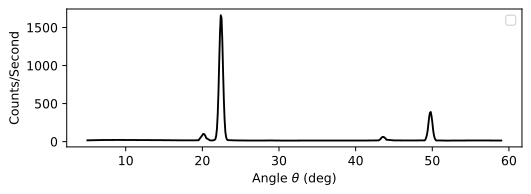
\includegraphics[scale=0.8]{lif.png}}
\caption{X-Ray diffraction pattern for $LiF$, between $\theta=5$ and $\theta=60$, using a time period of 3 seconds}
\label{fig:lif}
\end{figure}

From these observations, the angles at which the diffraction interference is constructive can be extracted. By writing the Bragg's law in terms of $d$ we obtain:

\begin{equation}
d=\frac{n\lambda}{2\sin\theta}
\end{equation}

From the plot, the peak wavelengths for $Cu-K_\alpha$ and $Cu-K_\beta$ were estimated, knowing that the $K_\alpha$ peak is the larger of the pair at each order. From these, one can obtain four estimates for $d$.

To estimate the error, using half of the measurement resolution, and propagating that through the equation, we use the following equation:
\begin{equation}
\sigma_d=d\cdot\sqrt{\left(\frac{\sigma_\theta}\theta\right)^2}
\end{equation}
Only the error for $\theta$ was included, as the wavelengths are given in the lab script, and the order has no error, as it is an integer.

\begin{table}[h!]
\centering
\begin{tabular}{ccccc}
\hline
Angle $(\deg)$ & Wavelength $(m)$ & Order & Estimate $(m)$ & Estimate Error $(\Delta m)$\\ \hline
20.15 & 1.392$\times10^{-10}$  & 1 & 2.021$\times10^{-10}$ & 1.076$\times10^{-11}$ \\
22.4 & 1.542$\times10^{-10}$ & 1 & 2.023$\times10^{-10}$ & 1.094$\times10^{-11}$ \\
43.55 & 1.392$\times10^{-10}$  & 2 & 2.021$\times10^{-10}$ & 1.394$\times10^{-11}$ \\
49.8  & 1.542$\times10^{-10}$ & 2 & 2.019$\times10^{-10}$ & 1.564$\times10^{-11}$ \\
\end{tabular}
\caption{\label{tab:liftab}Estimates for the $Cu-K_\beta$ and $Cu-K_\alpha$ interference peaks for $LiF$ diffraction, with the estimated value $d$ for lattice separation}
\end{table}

An estimate of $d=2.021\times10^{-10}\ m$ is obtained by averaging each of these estimates. To obtain an average error, we can divide the average by the root of the number of measurements, as repeated measurements reduce the overall error. An estimate error of $\sigma_d=6.41\times10^{-12}\ m$ was be calculated.

The lab simulation also provides a Nickel filter. Measurements were repeated at the same intervals, but this time with the Nickel filter in front of the X-Ray beam generator.

\begin{figure}[h]
\centerline{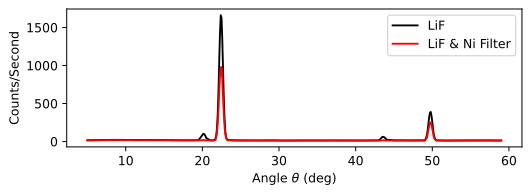
\includegraphics[scale=0.8]{lifni.png}}
\caption{X-Ray diffraction pattern for $LiF$, with and without the Nickel filter, between $\theta=5$ and $\theta=60$, using a time period of 3 seconds}
\label{fig:lifni}
\end{figure}

From this graph, one can see that the peaks corresponding to the $Cu-K_\alpha$ lines are reduced to around 60\% of their intensity without the filter, but the $Cu-K_\beta$ peaks are not present at all. This is explained by the Nickel atom's absorption edge at $1.448\r A$, which is between the $K_\alpha$ and $K_\beta$ lines. Therefore, this method can be used to distinguish $K_\alpha$ lines, present with a Nickel filter, from $K_\beta$ lines, which would not be present.

The same method can be repeated for NaCl\footnotemark[1], KCl\footnotemark[2], and RbCl\footnotemark[2] crystals.

\footnotetext[1]{Data obtained with permission from Sean Hibbit}
\footnotetext[2]{Data obtained with permission from Ethan Kosak-Hine}

\begin{figure}[h!]
\centerline{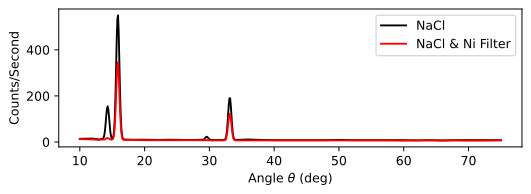
\includegraphics[scale=0.8]{nacl.png}}
\caption{X-Ray diffraction pattern for $NaCl$, with and without the Nickel filter, between $\theta=5$ and $\theta=60$, using a time period of 3 seconds}
\label{fig:nacl}
\end{figure}

\begin{table}[h!]
\centering
\begin{tabular}{ccccc}
\hline
Angle $(\deg)$ & Wavelength $(m)$ & Order & Estimate $(m)$ & Estimate Error $(\Delta m)$\\ \hline
14.3 & 1.392$\times10^{-10}$ & 1 & 2.818$\times10^{-10}$ & 1.454$\times10^{-11}$ \\
15.9 & 1.542$\times10^{-10}$ & 1 & 2.814$\times10^{-10}$ & 1.493$\times10^{-11}$ \\
29.6 & 1.392$\times10^{-10}$ & 2 & 2.818$\times10^{-10}$ & 1.620$\times10^{-11}$ \\
33.15 & 1.542$\times10^{-10}$ & 2 & 2.820$\times10^{-10}$ & 1.684$\times10^{-11}$ \\
\end{tabular}
\caption{\label{tab:nacltab}Estimates for the $Cu-K_\beta$ and $Cu-K_\alpha$ interference peaks for $NaCl$ diffraction, with the estimated value $d$ for lattice separation}
\end{table}

\begin{figure}[h!]
\centerline{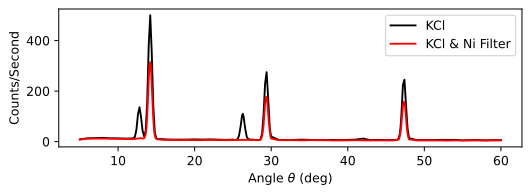
\includegraphics[scale=0.8]{kcl.png}}
\caption{X-Ray diffraction pattern for $KCl$, with and without the Nickel filter, between $\theta=5$ and $\theta=60$, using a time period of 3 seconds}
\label{fig:kcl}
\end{figure}

\begin{table}[h!]
\centering
\begin{tabular}{ccccc}
\hline
Angle $(\deg)$ & Wavelength $(m)$ & Order & Estimate $(m)$ & Estimate Error $(\Delta m)$\\ \hline
12.8 & 1.392$\times10^{-10}$ & 1 & 3.142$\times10^{-10}$ & 1.611$\times10^{-11}$ \\
14.2 & 1.542$\times10^{-10}$ & 1 & 3.143$\times10^{-10}$ & 1.621$\times10^{-11}$ \\
26.3 & 1.392$\times10^{-10}$  & 2 & 3.142$\times10^{-10}$ & 1.752$\times10^{-11}$ \\
29.3 & 1.542$\times10^{-10}$ & 2 & 3.151$\times10^{-10}$ & 1.807$\times10^{-11}$ \\
42 & 1.392$\times10^{-10}$  & 3 & 3.121$\times10^{-10}$ & 2.100$\times10^{-11}$ \\
47.3 & 1.542$\times10^{-10}$ & 3 & 3.147$\times10^{-10}$ & 2.320$\times10^{-11}$ \\
\end{tabular}
\caption{\label{tab:kcltab}Estimates for the $Cu-K_\beta$ and $Cu-K_\alpha$ interference peaks for $KCl$ diffraction, with the estimated value $d$ for lattice separation}
\end{table}

\begin{figure}[h!]
\centerline{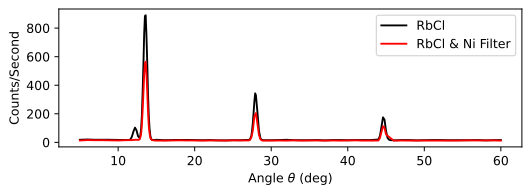
\includegraphics[scale=0.8]{rbcl.png}}
\caption{X-Ray diffraction pattern for $RbCl$, with and without the Nickel filter, between $\theta=5$ and $\theta=60$, using a time period of 3 seconds}
\label{fig:rbcl}
\end{figure}

\begin{table}[h!]
\centering
\begin{tabular}{ccccc}
\hline
Angle $(\deg)$ & Wavelength $(m)$ & Order & Estimate $(m)$ & Estimate Error $(\Delta m)$\\ \hline
12.1 & 1.392$\times10^{-10}$ & 1 & 3.320$\times10^{-10}$ & 1.698$\times10^{-11}$ \\
13.55 & 1.542$\times10^{-10}$ & 1 & 3.291$\times10^{-10}$ & 1.693$\times10^{-11}$ \\
27.9 & 1.542$\times10^{-10}$ & 2 & 3.295$\times10^{-10}$ & 1.864$\times10^{-11}$ \\
44.6 & 1.542$\times10^{-10}$ & 3 & 3.294$\times10^{-10}$ & 2.313$\times10^{-11}$ \\
\end{tabular}
\caption{\label{tab:rbcl}Estimates for the $Cu-K_\beta$ and $Cu-K_\alpha$ interference peaks for $RbCl$ diffraction, with the estimated value $d$ for lattice separation}
\end{table}
\newpage
\section{Conclusion}
From the same method as used with the $LiF$ crystal, we obtain the following averages:

\begin{table}[h!]
\centering
\begin{tabular}{ccc}
\hline
Crystal & Lattice Spacing Estimate $(m)$ & FCC Lattice Parameter $(m)$ \\ \hline
$LiF$ & $(2.021\pm0.0641)\times10^{-10}$ & $(4.042\pm0.128)\times10^{-10}$ \\
$NaCl$ & $(2.818\pm0.0781)\times10^{-10}$ & $(5.939\pm0.156)\times10^{-10}$ \\
$KCl$ & $(3.141\pm0.0763)\times10^{-10}$ & $(6.282\pm0.153)\times10^{-10}$ \\
$RbCl$ & $(3.300\pm0.0946)\times10^{-10}$ & $(6.600\pm0.189)\times10^{-10}$ \\
\end{tabular}
\caption{\label{tab:results}Estimated values $d$ for lattice separation for crystals $LiF$, $NaCl$, $KCl$, and $RbCl$, with error ranges, and Face-Centered-Cubic lattice parameter $a=2d$.}
\end{table}

As the $LiF$ crystal contains $F^-$ ions, whereas the other three crystals contain $CL^-$ ions, we cannot directly relate the size of the $LiF$ lattice parameter to the $Li^+$ ion size. However, as the other three crystals contain $Cl^-$ ions, we can factor their size out, and compare the $Na^+$, $K^+$, and $Rb^+$ ion sizes with known values taken from Kittel, C. {\it Introduction to Solid State Physics} (8 ed.).

\begin{flushright}
{\it Cont. overleaf.}
\end{flushright}
\newpage
\begin{table}[h!]
\centering
\begin{tabular}{ccccc}
\hline
Ion & Lattice spacing $(m\times10^{-10})$ & Relative size & Known size $(\r A)$ & Known relative size \\ \hline
$Na^+$ & $2.818 \pm 0.0781$ & 1 & 0.98 & 1 \\
$K^+$ & $3.141\pm0.0763$ & 1.115 & 1.33 & 1.357 \\
$Rb^+$ & $3.3\pm0.0946$ & 1.171 & 1.48 & 1.510 \\
\end{tabular}
\caption{\label{tab:comparison}Comparing the calculated relative sizes of $Na^+$, $K^+$, and $Rb^+$ ions to known values.}
\end{table}

While these calculated relative sizes (relative to $Na^+$) do not perfectly line up to the known relative sizes, it is promising to see the expected increase. From looking at a periodic table, we see that $Na$, $K$, and $Rb$ are alkali metals of increasing electron configuration, and we would expect $Li^+$ ions to follow the trend, being smaller than $Na^+$, but we cannot conclude this due to the $F$ anion, rather than $Cl$ in the rest of the crystals. We can expect a linear progression of ion size, as each increasing electron orbital can be estimated to be the same size. 

\end{document}
